% ============================================================
%  Relatório Técnico — Modelo da Planta AEB
%  Compilar com: tectonic relatorio_planta.tex
% ============================================================
\documentclass[12pt,a4paper]{article}

% --- Codificação e língua ----------------------------------------
\usepackage[utf8]{inputenc}
\usepackage[T1]{fontenc}
\usepackage[brazil]{babel}

% --- Tipografia --------------------------------------------------
\usepackage{lmodern}
\usepackage{microtype}

% --- Layout ------------------------------------------------------
\usepackage[
  top=2.5cm, bottom=2.5cm,
  left=2.8cm, right=2.8cm,
  headheight=15pt
]{geometry}
\usepackage{fancyhdr}
\usepackage{titlesec}
\usepackage{parskip}
\setlength{\parindent}{0pt}
\setlength{\parskip}{6pt}

% --- Cor e links -------------------------------------------------
\usepackage{xcolor}
\definecolor{azulescuro}{RGB}{30,60,100}
\definecolor{azulmedio}{RGB}{52,100,160}
\definecolor{azulclaro}{RGB}{220,235,250}
\definecolor{cinzatexto}{RGB}{80,80,80}
\definecolor{verdedest}{RGB}{27,94,32}
\definecolor{amarelodest}{RGB}{255,243,205}
\definecolor{amarelob}{RGB}{180,130,0}
\definecolor{laranjacode}{RGB}{200,80,0}

\usepackage[
  colorlinks=true,
  linkcolor=azulmedio,
  urlcolor=azulmedio,
  citecolor=azulmedio
]{hyperref}

% --- Figuras e tabelas -------------------------------------------
\usepackage{graphicx}
\usepackage{float}
\usepackage{caption}
\usepackage{subcaption}
\usepackage{booktabs}
\usepackage{array}
\usepackage{colortbl}
\usepackage{longtable}
\usepackage{tabularx}

% --- Caixas e destaques ------------------------------------------
\usepackage{tcolorbox}
\tcbuselibrary{skins,breakable}

\newtcolorbox{notabox}[1][]{
  colback=amarelodest, colframe=amarelob,
  fonttitle=\bfseries\small, title=#1,
  left=4pt, right=4pt, top=3pt, bottom=3pt,
  breakable
}

\newtcolorbox{codigobox}{
  colback=gray!10, colframe=gray!40,
  fontupper=\ttfamily\small,
  left=8pt, right=4pt, top=4pt, bottom=4pt,
  breakable
}

\newtcolorbox{equacaobox}{
  colback=azulclaro, colframe=azulmedio,
  fontupper=\large\bfseries,
  halign=center,
  left=4pt, right=4pt, top=6pt, bottom=6pt
}

% --- Matemática --------------------------------------------------
\usepackage{amsmath}
\usepackage{amssymb}

% --- Código ------------------------------------------------------
\usepackage{listings}
\lstset{
  basicstyle=\ttfamily\footnotesize,
  keywordstyle=\color{azulmedio}\bfseries,
  stringstyle=\color{verdedest},
  commentstyle=\color{cinzatexto}\itshape,
  backgroundcolor=\color{gray!8},
  frame=single,
  framerule=0.4pt,
  rulecolor=\color{gray!40},
  numbers=left,
  numberstyle=\tiny\color{gray},
  numbersep=8pt,
  breaklines=true,
  showstringspaces=false,
  language=Matlab
}

% --- Cabeçalho e rodapé ------------------------------------------
\pagestyle{fancy}
\fancyhf{}
\fancyhead[L]{\small\color{cinzatexto}Modelo da Planta AEB}
\fancyhead[R]{\small\color{cinzatexto}Documentação Técnica}
\fancyfoot[C]{\small\color{cinzatexto}\thepage}
\renewcommand{\headrulewidth}{0.4pt}
\renewcommand{\headrule}{\hbox to\headwidth{\color{azulmedio}\leaders\hrule height \headrulewidth\hfill}}

% --- Títulos de seção --------------------------------------------
\titleformat{\section}
  {\Large\bfseries\color{azulescuro}}
  {\thesection.}{0.6em}{}
  [\color{azulmedio}\rule{\linewidth}{1.2pt}]

\titleformat{\subsection}
  {\large\bfseries\color{azulmedio}}
  {\thesubsection}{0.6em}{}

\titleformat{\subsubsection}
  {\normalsize\bfseries\color{azulescuro}}
  {\thesubsubsection}{0.5em}{}

% --- Captions ----------------------------------------------------
\captionsetup{
  font=small,
  labelfont={bf,color=azulescuro},
  textfont={color=cinzatexto},
  margin=10pt
}

% --- Macro para parâmetro ----------------------------------------
\newcommand{\param}[1]{\texttt{\color{laranjacode}#1}}
\newcommand{\unid}[1]{\text{~[#1]}}

% ================================================================
\begin{document}

% --- Capa --------------------------------------------------------
\begin{titlepage}
  \pagecolor{azulescuro}
  \color{white}
  \vspace*{2cm}

  \begin{center}
    {\fontsize{11}{13}\selectfont\scshape Projeto AEB --- Pós-Graduação em Engenharia Automotiva}\\[0.8cm]
    \rule{\linewidth}{1.5pt}\\[0.6cm]
    {\fontsize{28}{34}\selectfont\bfseries Modelo da Planta\\do Sistema AEB}\\[0.4cm]
    \rule{\linewidth}{1.5pt}\\[0.8cm]
    {\fontsize{15}{18}\selectfont Documentação Técnica e Justificativa de Parâmetros}\\[0.3cm]
    {\fontsize{12}{15}\selectfont\color{azulclaro}%
      Autonomous Emergency Braking --- Simulink Plant Model}\\[2.5cm]
  \end{center}

  \begin{tcolorbox}[
    colback=azulmedio!60!azulescuro,
    colframe=white!40!azulmedio,
    fontupper=\color{white},
    left=10pt, right=10pt, top=8pt, bottom=8pt
  ]
    \begin{tabular}{ll}
      \textbf{Versão}          & 1.0 \\[3pt]
      \textbf{Data}            & Março de 2026 \\[3pt]
      \textbf{Referência}      & \texttt{modeling/AEB\_Plant\_build.m} \\[3pt]
      \textbf{Compatibilidade} & MATLAB/Simulink R2025b \\[3pt]
      \textbf{Normas}          & Euro NCAP AEB C2C v4.3 $\cdot$ UNECE R152 $\cdot$ SAE J2452 \\
    \end{tabular}
  \end{tcolorbox}

  \vfill
  \begin{center}
    {\small\color{azulclaro}%
      Gerado por \texttt{AEB\_Plant\_build.m} ---
      Figuras por \texttt{gerar\_figs.py}}
  \end{center}
\end{titlepage}

\pagecolor{white}
\color{black}

% --- Sumário -----------------------------------------------------
\tableofcontents
\newpage

% ================================================================
\section{Visão Geral do Modelo}
\label{sec:visao}

O modelo da planta representa o \textbf{ambiente físico} no qual o sistema AEB opera.
Ao contrário do controlador --- que implementa a lógica de decisão na FSM ---,
a planta modela o mundo físico: o comportamento dinâmico do veículo ego, a resposta
do atuador de freio, o movimento do veículo-alvo e a evolução da distância entre eles.

O modelo foi desenvolvido com foco em simulação \textbf{Software-in-the-Loop (SIL)},
sendo suficientemente fiel para validar o comportamento do controlador AEB embarcado
em C (\texttt{c\_embedded/}), sem complexidade desnecessária.

\begin{notabox}[Operação independente]
O modelo é autossuficiente: inclui um sinal de teste interno (degrau de 5\,bar em
$t = 3$\,s) controlado por um \emph{Manual Switch}. Basta executar
\texttt{sim('AEB\_Plant')} sem nenhum controlador conectado para verificar
imediatamente a resposta dinâmica do veículo e do atuador.
\end{notabox}

\subsection{Estrutura em quatro subsistemas}

\begin{figure}[H]
  \centering
  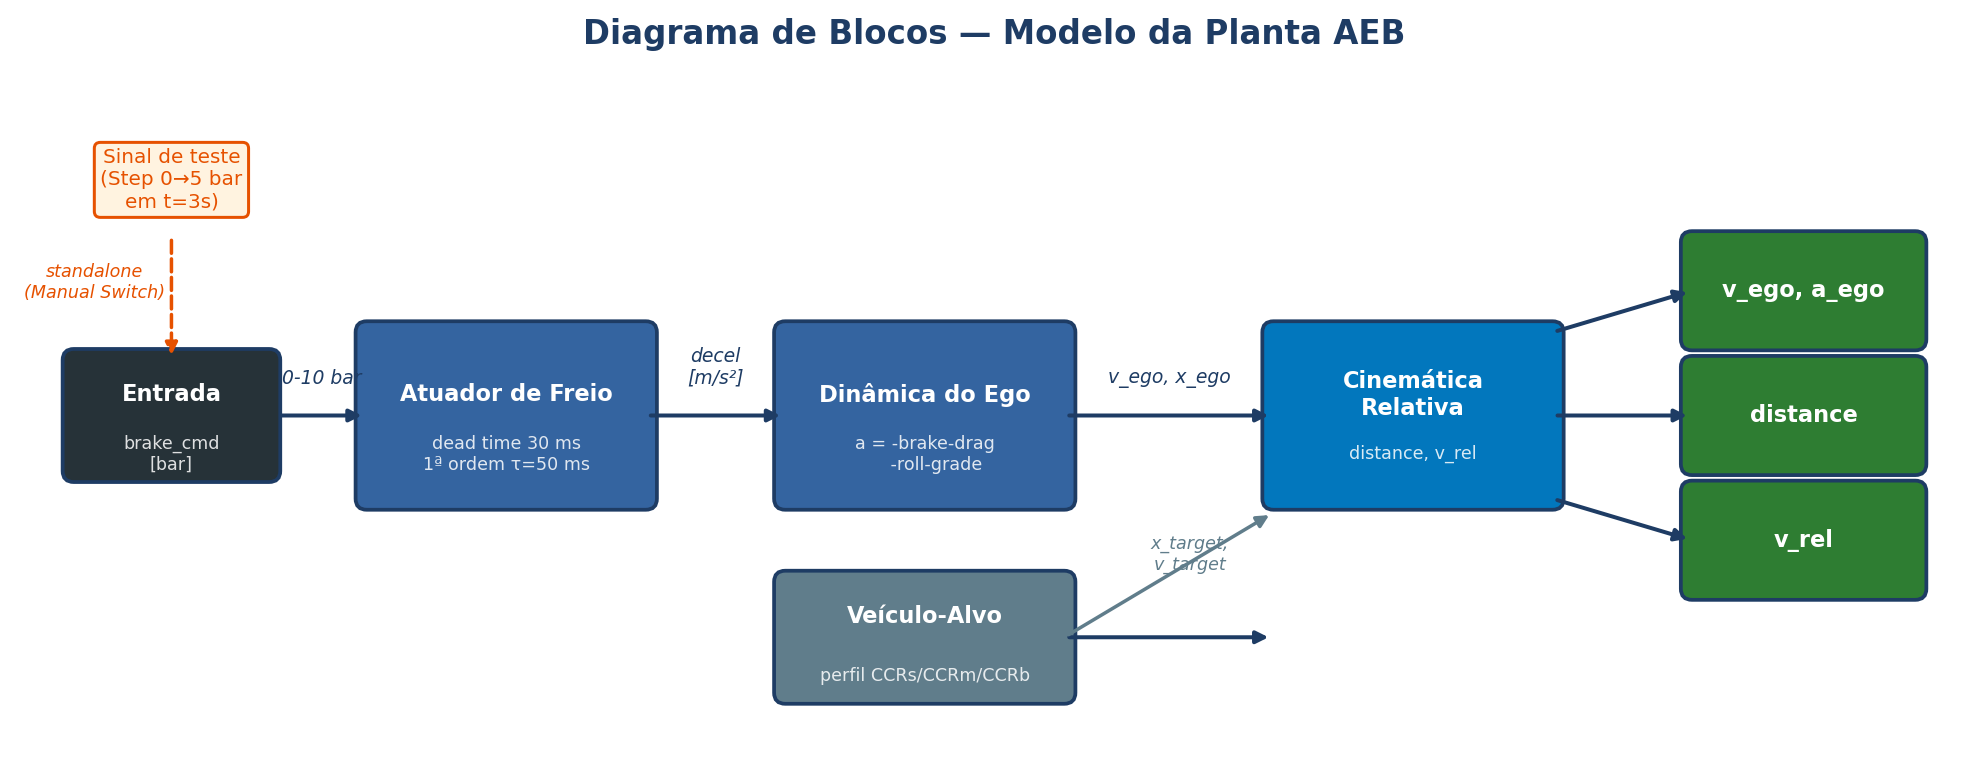
\includegraphics[width=\linewidth]{figs/fig_blocos.png}
  \caption{Diagrama de blocos do Modelo da Planta AEB com entradas, saídas e subsistemas.}
  \label{fig:blocos}
\end{figure}

O modelo é composto por quatro subsistemas interconectados (Figura~\ref{fig:blocos}):

\begin{enumerate}
  \item \textbf{Atuador de Freio} --- transforma o comando de pressão (0--10\,bar) em
        desaceleração efetiva, aplicando atraso de transporte (30\,ms) e dinâmica de
        1\textsuperscript{a} ordem ($\tau = 50$\,ms).

  \item \textbf{Dinâmica do Ego} --- recebe a desaceleração do atuador e calcula a
        aceleração resultante, integrando para obter velocidade e posição. Inclui
        arrasto aerodinâmico, resistência ao rolamento e inclinação da via.

  \item \textbf{Perfil do Veículo-Alvo} --- gera a velocidade e posição do alvo com base
        no cenário selecionado (CCRs, CCRm, CCRb). Suporta alvo estacionário, em
        movimento constante ou desacelerando a partir de um instante definido.

  \item \textbf{Cinemática Relativa} --- calcula distância inter-veicular, velocidade
        relativa e detecta colisão. Estes sinais são as saídas primárias consumidas
        pelo controlador via CAN.
\end{enumerate}

\subsection{Entradas e saídas}

\begin{table}[H]
  \centering
  \caption{Entradas do modelo da planta.}
  \begin{tabularx}{\linewidth}{lllX}
    \toprule
    \rowcolor{azulescuro!90}
    \color{white}\textbf{Sinal} &
    \color{white}\textbf{Unidade} &
    \color{white}\textbf{Modo} &
    \color{white}\textbf{Descrição} \\
    \midrule
    \param{brake\_cmd\_bar} & bar (0--10) & Externo & Pressão comandada pelo controlador AEB \\
    \rowcolor{azulclaro!50}
    \param{brake\_cmd\_bar} & bar (0--10) & Interno & Degrau de teste (0$	o$5\,bar em $t = 3$\,s) \\
    \bottomrule
  \end{tabularx}
\end{table}

\begin{table}[H]
  \centering
  \caption{Saídas do modelo da planta.}
  \begin{tabularx}{\linewidth}{lllX}
    \toprule
    \rowcolor{azulescuro!90}
    \color{white}\textbf{Sinal} &
    \color{white}\textbf{Unidade} &
    \color{white}\textbf{Destino} &
    \color{white}\textbf{Descrição} \\
    \midrule
    \param{ego\_speed}    & m/s   & CAN 0x100 & Velocidade do ego \\
    \rowcolor{azulclaro!50}
    \param{ego\_accel}    & m/s²  & CAN 0x100 & Aceleração do ego \\
    \param{target\_speed} & m/s   & Interno   & Velocidade do alvo \\
    \rowcolor{azulclaro!50}
    \param{distance}      & m     & CAN 0x120 & Distância inter-veicular \\
    \param{rel\_speed}    & m/s   & CAN 0x120 & Velocidade relativa \\
    \rowcolor{azulclaro!50}
    \param{collision}     & bool  & Dashboard & Colisão detectada ($d \leq 0{,}5$\,m) \\
    \bottomrule
  \end{tabularx}
\end{table}

% ================================================================
\section{Processo de Construção do Modelo em Simulink}
\label{sec:processo}

\subsection{Pré-requisitos}

\begin{itemize}
  \item MATLAB R2025b (compatível com R2024b ou superior)
  \item Simulink (toolbox base --- \emph{sem toolboxes adicionais})
  \item Pasta de trabalho: \texttt{C:\textbackslash Users\textbackslash rfagu\textbackslash Codigos\textbackslash Pos\textbackslash AEB\textbackslash modeling\textbackslash}
\end{itemize}

\begin{notabox}[Toolboxes necessários]
Nenhum toolbox adicional é necessário. O modelo usa apenas a biblioteca padrão
do Simulink: blocos \emph{Continuous}, \emph{Math Operations},
\emph{Signal Routing}, \emph{Sources} e \emph{Sinks}.
\end{notabox}

\subsection{Sequência de execução}

\begin{figure}[H]
  \centering
  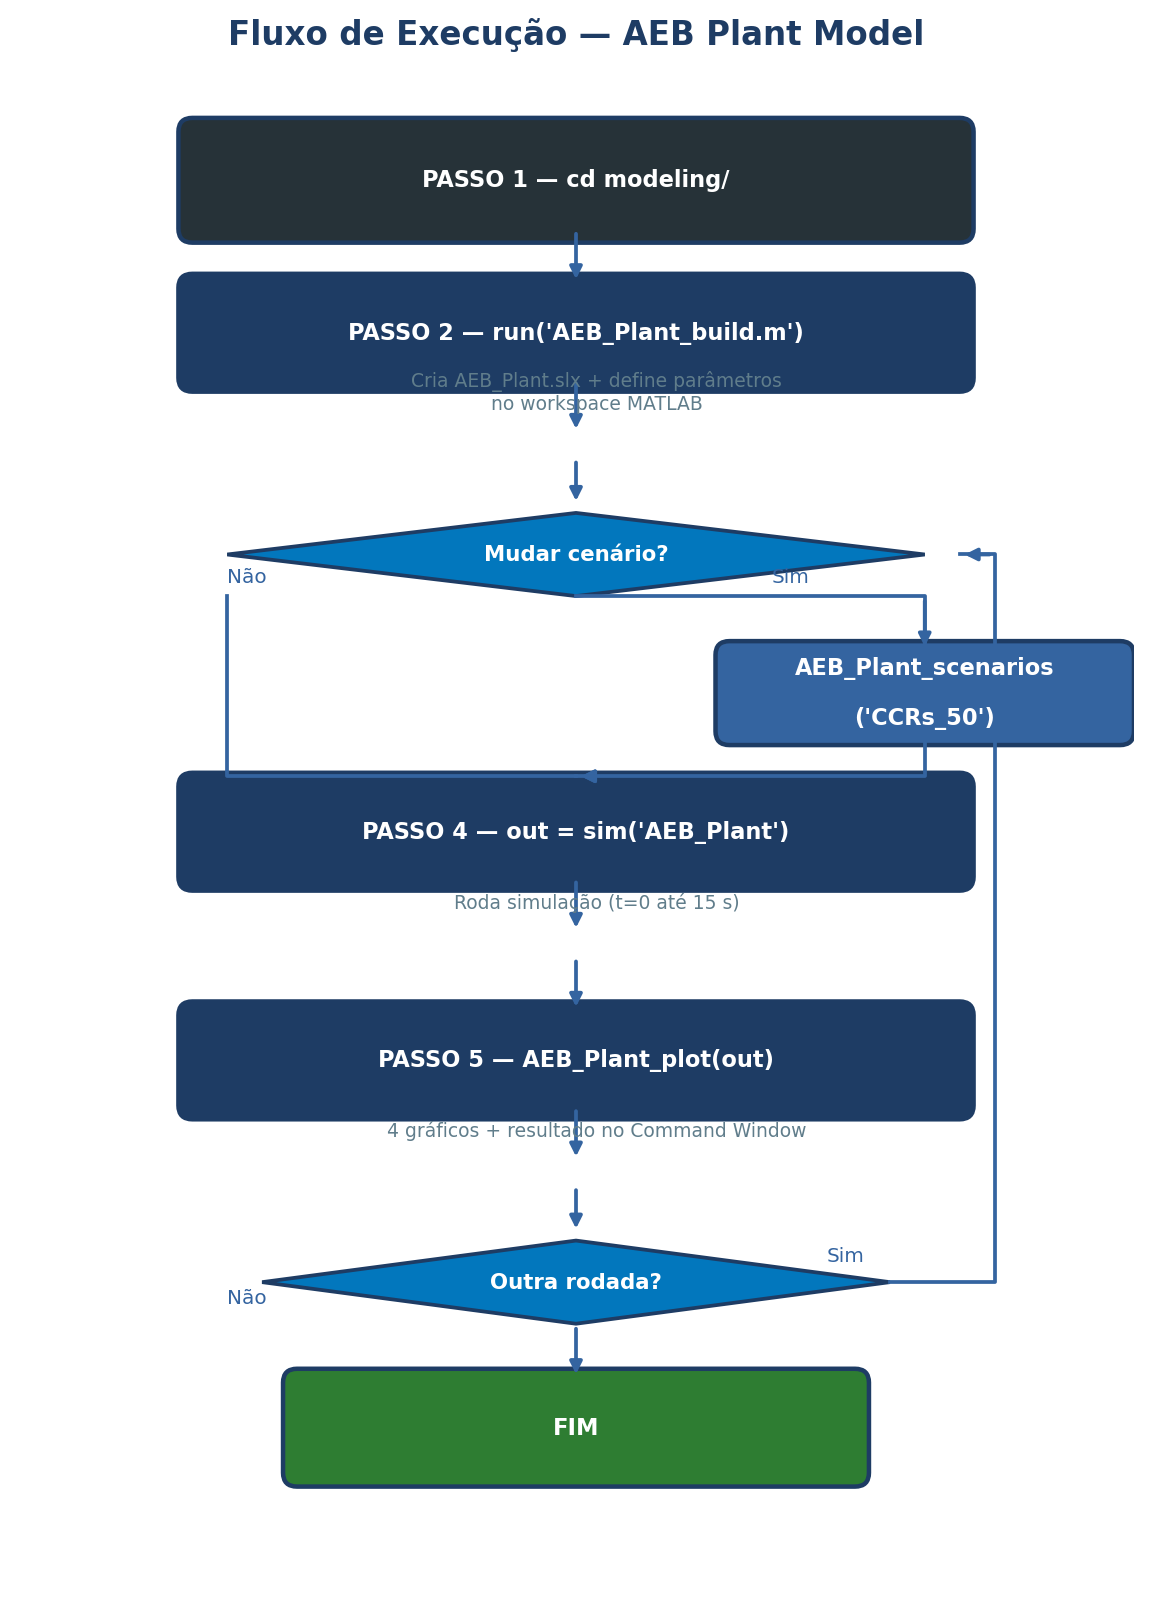
\includegraphics[width=0.72\linewidth]{figs/fig_fluxo.png}
  \caption{Fluxo completo de execução do modelo, do ambiente MATLAB até a análise dos resultados.}
  \label{fig:fluxo}
\end{figure}

O modelo é gerado inteiramente por script MATLAB, sem interação manual com a interface
gráfica do Simulink. A sequência completa é apresentada na Figura~\ref{fig:fluxo} e
detalhada abaixo:

\subsubsection*{Passo 1 --- Navegar para a pasta do projeto}
\begin{codigobox}
cd 'C:\textbackslash Users\textbackslash rfagu\textbackslash Codigos\textbackslash Pos\textbackslash AEB\textbackslash modeling'
\end{codigobox}

\subsubsection*{Passo 2 --- Executar o script de construção}
\begin{codigobox}
run('AEB\_Plant\_build.m')
\end{codigobox}
Cria o modelo \texttt{AEB\_Plant.slx}, define todos os parâmetros no workspace MATLAB
e salva o arquivo. O script leva aproximadamente 5 segundos e exibe confirmação no
\emph{Command Window}.

\subsubsection*{Passo 3 --- (Opcional) Selecionar cenário}
\begin{codigobox}
AEB\_Plant\_scenarios('CCRs\_50')
\end{codigobox}
Atualiza as variáveis \param{SCENARIO\_*} no workspace.
Cenários disponíveis: \texttt{CCRs\_20}, \texttt{CCRs\_30}, \texttt{CCRs\_40},
\texttt{CCRs\_50}, \texttt{CCRm}, \texttt{CCRb}, \texttt{CCRb\_hard}, \texttt{no\_aeb}.

\subsubsection*{Passo 4 --- Executar a simulação}
\begin{codigobox}
out = sim('AEB\_Plant');
\end{codigobox}
Executa a simulação com os parâmetros atuais. Retorna um objeto \texttt{SimulationOutput}.

\subsubsection*{Passo 5 --- Visualizar resultados}
\begin{codigobox}
AEB\_Plant\_plot(out)
\end{codigobox}
Plota 4 gráficos (velocidades, distância, velocidade relativa, aceleração) e
imprime o resultado (colisão ou parada) no \emph{Command Window}.

\subsection{Blocos Simulink utilizados}

\begin{table}[H]
  \centering
  \caption{Blocos Simulink empregados no modelo da planta e suas funções.}
  \begin{tabularx}{\linewidth}{llX}
    \toprule
    \rowcolor{azulescuro!90}
    \color{white}\textbf{Bloco} &
    \color{white}\textbf{Biblioteca} &
    \color{white}\textbf{Função no modelo} \\
    \midrule
    \texttt{Gain}              & Math Operations  & Converte bar $\to$ normalizado e normalizado $\to$ m/s² \\
    \rowcolor{azulclaro!50}
    \texttt{Transport Delay}   & Continuous       & Atraso hidráulico do atuador (30\,ms) \\
    \texttt{Transfer Fcn}      & Continuous       & Dinâmica de 1\textsuperscript{a} ordem do atuador ($\tau = 50$\,ms) \\
    \rowcolor{azulclaro!50}
    \texttt{Saturation}        & Discontinuities  & Limita desaceleração (0--10\,m/s²) e velocidade ($v \geq 0$) \\
    \texttt{Integrator}        & Continuous       & Integra aceleração $\to$ velocidade e velocidade $\to$ posição \\
    \rowcolor{azulclaro!50}
    \texttt{Math Function}     & Math Operations  & Calcula $v^2$ para o arrasto aerodinâmico \\
    \texttt{Constant}          & Sources          & Parâmetros de cenário e resistências do veículo \\
    \rowcolor{azulclaro!50}
    \texttt{Sum}               & Math Operations  & Soma de forças; diferença de posições e velocidades \\
    \texttt{Clock}             & Sources          & Tempo para detectar o instante de frenagem do alvo \\
    \rowcolor{azulclaro!50}
    \texttt{Manual Switch}     & Signal Routing   & Seleciona entrada de freio (teste interno vs.\ externo) \\
    \texttt{Step}              & Sources          & Sinal de teste: 0 $\to$ 5\,bar em $t = 3$\,s \\
    \rowcolor{azulclaro!50}
    \texttt{To Workspace}      & Sinks            & Registra sinais para análise pós-simulação \\
    \texttt{Scope}             & Sinks            & Visualização em tempo real (4 sinais) \\
    \bottomrule
  \end{tabularx}
\end{table}

\subsection{Modo standalone (sem controlador)}

O modelo permite execução completamente independente por meio de um bloco
\emph{Manual Switch} que chaveie entre dois modos:

\begin{itemize}
  \item \textbf{Posição 1 (padrão após o build)}: sinal interno de degrau ---
        0 $\to$ 5\,bar em $t = 3$\,s, representando um comando BRAKE\_L2.
        Permite observar a resposta do atuador e a desaceleração resultante
        sem nenhum arquivo externo ou controlador.

  \item \textbf{Posição 2}: entrada externa via porta \param{brake\_cmd\_bar} ---
        usada quando o controlador AEB (\texttt{AEB\_Stateflow.slx}) está
        conectado em modo integrado.
\end{itemize}

Para alternar: abra \texttt{AEB\_Plant.slx} e clique duas vezes no bloco
\texttt{InputSelect}.

% ================================================================
\section{Parâmetros do Veículo}
\label{sec:params}

\begin{figure}[H]
  \centering
  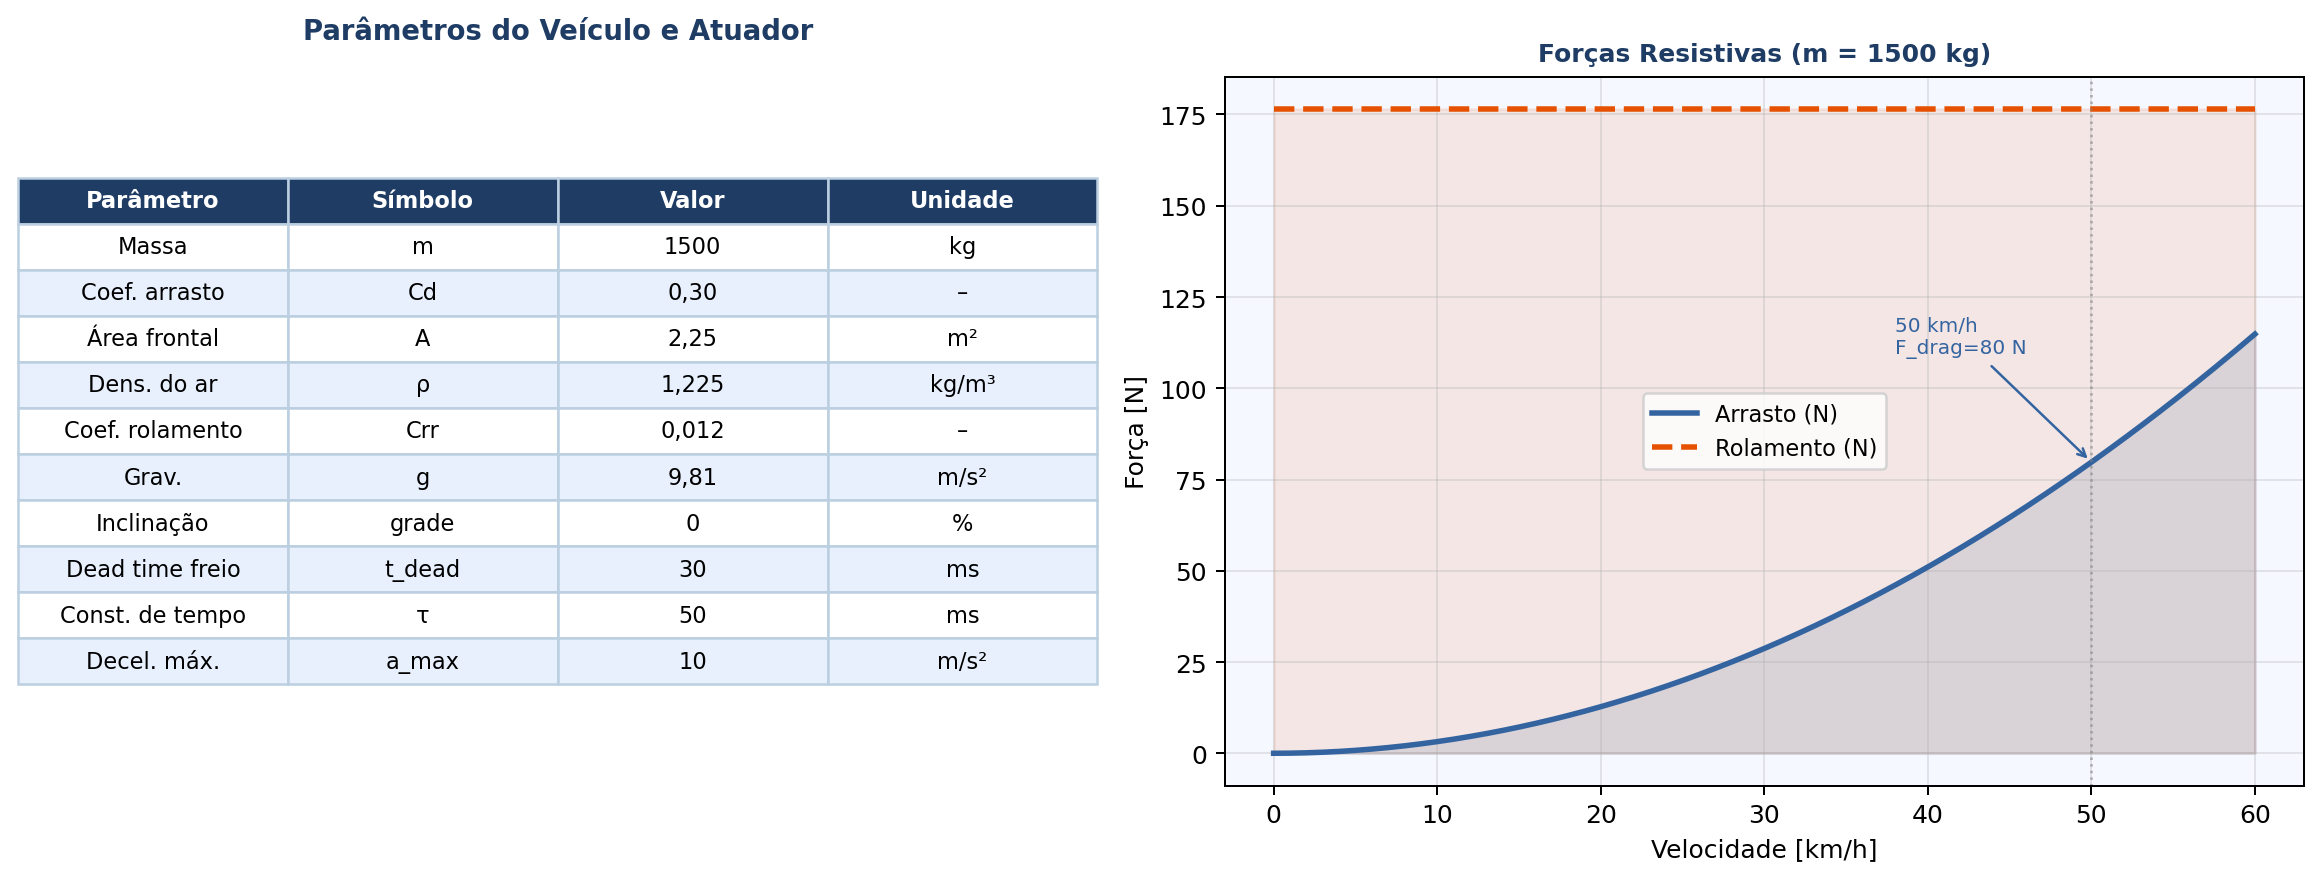
\includegraphics[width=\linewidth]{figs/fig_params.png}
  \caption{Tabela de parâmetros (esq.) e forças resistivas em função da velocidade (dir.).}
  \label{fig:params}
\end{figure}

\subsection{Massa do veículo}

\begin{table}[H]
  \centering
  \begin{tabular}{lccc}
    \toprule
    \rowcolor{azulescuro!90}
    \color{white}\textbf{Variável} & \color{white}\textbf{Valor} &
    \color{white}\textbf{Unidade} & \color{white}\textbf{Faixa típica} \\
    \midrule
    \param{VEHICLE\_MASS} & 1500 & kg & 1300--1500 \\
    \bottomrule
  \end{tabular}
\end{table}

Valor representativo de um sedã compacto utilizado em testes Euro NCAP (VW Golf,
Hyundai i30, Opel Astra). A massa inclui o veículo em ordem de marcha com 75\,kg
de carga representando o condutor.

\textbf{Fonte:} Euro NCAP AEB C2C Test Protocol v4.3; MathWorks AEB Test Bench.

\subsection{Aerodinâmica}

\begin{table}[H]
  \centering
  \begin{tabular}{lcccc}
    \toprule
    \rowcolor{azulescuro!90}
    \color{white}\textbf{Variável} & \color{white}\textbf{Valor} &
    \color{white}\textbf{Unidade} & \color{white}\textbf{Faixa} & \color{white}\textbf{Referência} \\
    \midrule
    \param{Cd}        & 0,30  & ---    & 0,25--0,35 & Média sedã compacto \\
    \rowcolor{azulclaro!50}
    \param{A\_FRONTAL} & 2,25  & m²     & 2,10--2,50 & Classe compacto \\
    \param{RHO\_AIR}  & 1,225 & kg/m³  & ---        & ISA, 15°C, nível do mar \\
    \bottomrule
  \end{tabular}
\end{table}

A força de arrasto é $F_\text{drag} = \tfrac{1}{2}\, C_d \cdot A \cdot \rho \cdot v^2$.
A 50\,km/h, $F_\text{drag} \approx 40$\,N (desaceleração de 0,027\,m/s²) --- contribuição
marginal nos cenários AEB de curta duração, mas incluída por completude.

\subsection{Resistência ao rolamento}

\begin{table}[H]
  \centering
  \begin{tabular}{lccc}
    \toprule
    \rowcolor{azulescuro!90}
    \color{white}\textbf{Variável} & \color{white}\textbf{Valor} &
    \color{white}\textbf{Unidade} & \color{white}\textbf{Faixa (SAE J2452)} \\
    \midrule
    \param{Crr} & 0,012 & --- & 0,006--0,015 \\
    \bottomrule
  \end{tabular}
\end{table}

Coeficiente de resistência ao rolamento para pneus de passageiros em asfalto seco
(40--60\,km/h). Desaceleração resultante: $C_{rr} \cdot g = 0{,}012 \times 9{,}81 = 0{,}118$\,m/s².

\textbf{Fonte:} SAE J2452.

\subsection{Inclinação da via}

Valor de referência: $\text{grade} = 0$\% (superfície plana, conforme protocolo Euro NCAP).
O parâmetro \param{ROAD\_GRADE} é configurável para análise de robustez ($\pm 6$\%).

% ================================================================
\section{Parâmetros do Atuador de Freio}
\label{sec:atuador}

\begin{figure}[H]
  \centering
  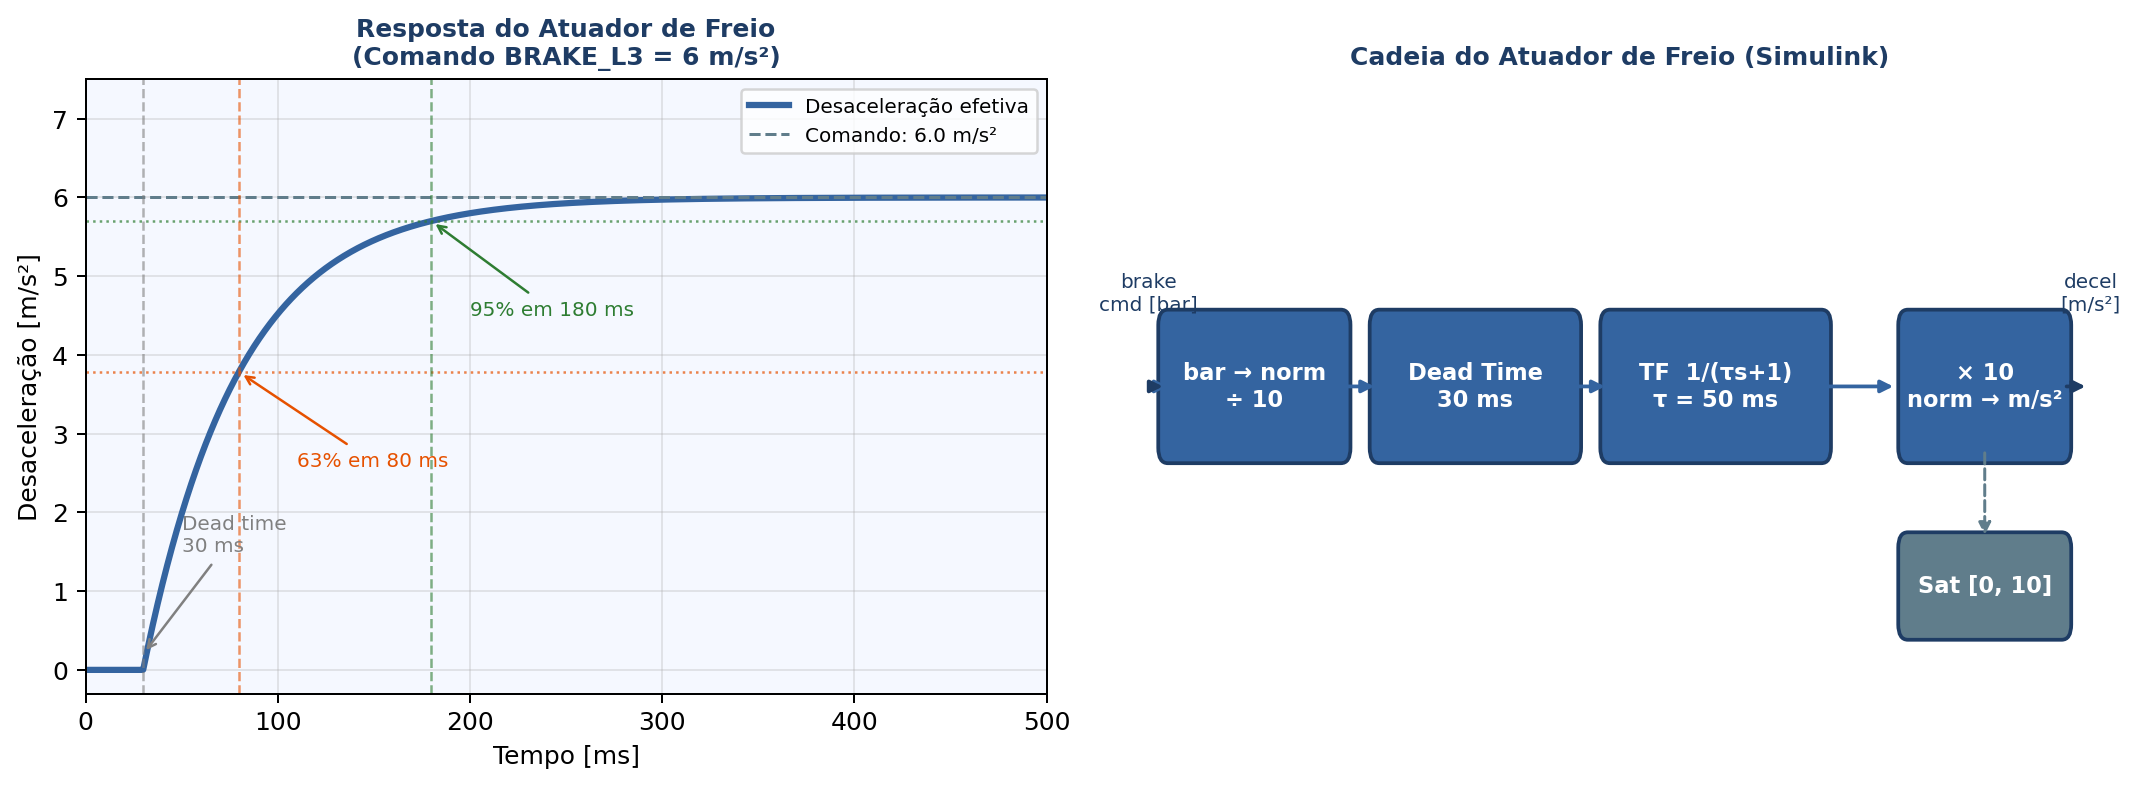
\includegraphics[width=\linewidth]{figs/fig_atuador.png}
  \caption{Resposta temporal do atuador (esq.) e cadeia de blocos Simulink (dir.).}
  \label{fig:atuador}
\end{figure}

\subsection{Modelo do atuador}

O atuador é modelado como um sistema de 1\textsuperscript{a} ordem com atraso de
transporte, representando a dinâmica hidráulica entre o comando elétrico e a pressão
efetiva nas pastilhas:

\begin{equacaobox}
$G(s) = e^{-s \cdot t_\text{dead}} \cdot \dfrac{1}{\tau s + 1}$
\end{equacaobox}

\begin{table}[H]
  \centering
  \caption{Parâmetros do atuador de freio.}
  \begin{tabularx}{\linewidth}{lccX}
    \toprule
    \rowcolor{azulescuro!90}
    \color{white}\textbf{Variável} & \color{white}\textbf{Valor} &
    \color{white}\textbf{Unidade} & \color{white}\textbf{Justificativa} \\
    \midrule
    \param{BRAKE\_DEAD\_TIME} & 30  & ms    & Atraso hidráulico ESC/iBooster (faixa: 30--100\,ms) \\
    \rowcolor{azulclaro!50}
    \param{BRAKE\_TAU}        & 50  & ms    & Constante de tempo de pressurização (0$	o$63\% em 50\,ms) \\
    \param{BRAKE\_MAX\_DECEL} & 10  & m/s²  & Capacidade máxima ($\mu \cdot g \approx 8{,}3$ + arrasto) \\
    \rowcolor{azulclaro!50}
    \param{BRAKE\_BAR\_MAX}   & 10  & bar   & Pressão máxima mapeada para 10\,m/s² (linear) \\
    \bottomrule
  \end{tabularx}
\end{table}

\subsection{Resposta temporal}

\begin{table}[H]
  \centering
  \caption{Métricas de resposta para comando BRAKE\_L3 (6\,m/s²).}
  \begin{tabular}{lll}
    \toprule
    \rowcolor{azulescuro!90}
    \color{white}\textbf{Métrica} & \color{white}\textbf{Tempo} & \color{white}\textbf{Cálculo} \\
    \midrule
    Início da resposta & 30\,ms  & $t_\text{dead}$ \\
    \rowcolor{azulclaro!50}
    63\% do valor final & 80\,ms  & $t_\text{dead} + \tau$ \\
    90\% do valor final & 145\,ms & $t_\text{dead} + 2{,}3\,\tau$ \\
    \rowcolor{azulclaro!50}
    95\% do valor final & 180\,ms & $t_\text{dead} + 3\,\tau$ \\
    \bottomrule
  \end{tabular}
\end{table}

A 50\,km/h, os 180\,ms do transitório correspondem a $\approx 2{,}5$\,m percorridos
antes de atingir 95\% da desaceleração comandada --- distância relevante para o
dimensionamento dos limiares de TTC da FSM.

\textbf{Fonte:} Bosch iBooster datasheet; \texttt{aeb\_config.h}: \param{BRAKE\_DEAD\_TIME = 0.03f}, \param{BRAKE\_TAU = 0.05f}.

% ================================================================
\section{Coeficiente de Atrito Pneu-Estrada}
\label{sec:atrito}

\begin{table}[H]
  \centering
  \begin{tabular}{lcll}
    \toprule
    \rowcolor{azulescuro!90}
    \color{white}\textbf{Parâmetro} & \color{white}\textbf{Valor} &
    \color{white}\textbf{Como é usado} & \color{white}\textbf{Condição} \\
    \midrule
    $\mu$ (implícito) & 0,85 & Limita \param{BRAKE\_MAX\_DECEL} & Asfalto seco \\
    \rowcolor{azulclaro!50}
    $\mu$ (chuva)     & $\sim$0,5 & Reduzir \param{BRAKE\_MAX\_DECEL} & Condição adversa \\
    $\mu$ (neve)      & $\sim$0,2 & Reduzir \param{BRAKE\_MAX\_DECEL} & Condição severa \\
    \bottomrule
  \end{tabular}
\end{table}

O coeficiente de atrito pico em asfalto seco para pneus de passageiros é tipicamente
0,80--0,91. O valor é implícito no modelo via \param{BRAKE\_MAX\_DECEL}: $\mu \times g \approx 0{,}85 \times 9{,}81 \approx 8{,}3$\,m/s², acrescido da contribuição de arrasto e rolamento para totalizar 10\,m/s².

\textbf{Fonte:} Taylor \& Francis --- Tire-Road Friction Estimation (2014).

% ================================================================
\section{Cenários de Simulação (Euro NCAP)}
\label{sec:cenarios}

\begin{figure}[H]
  \centering
  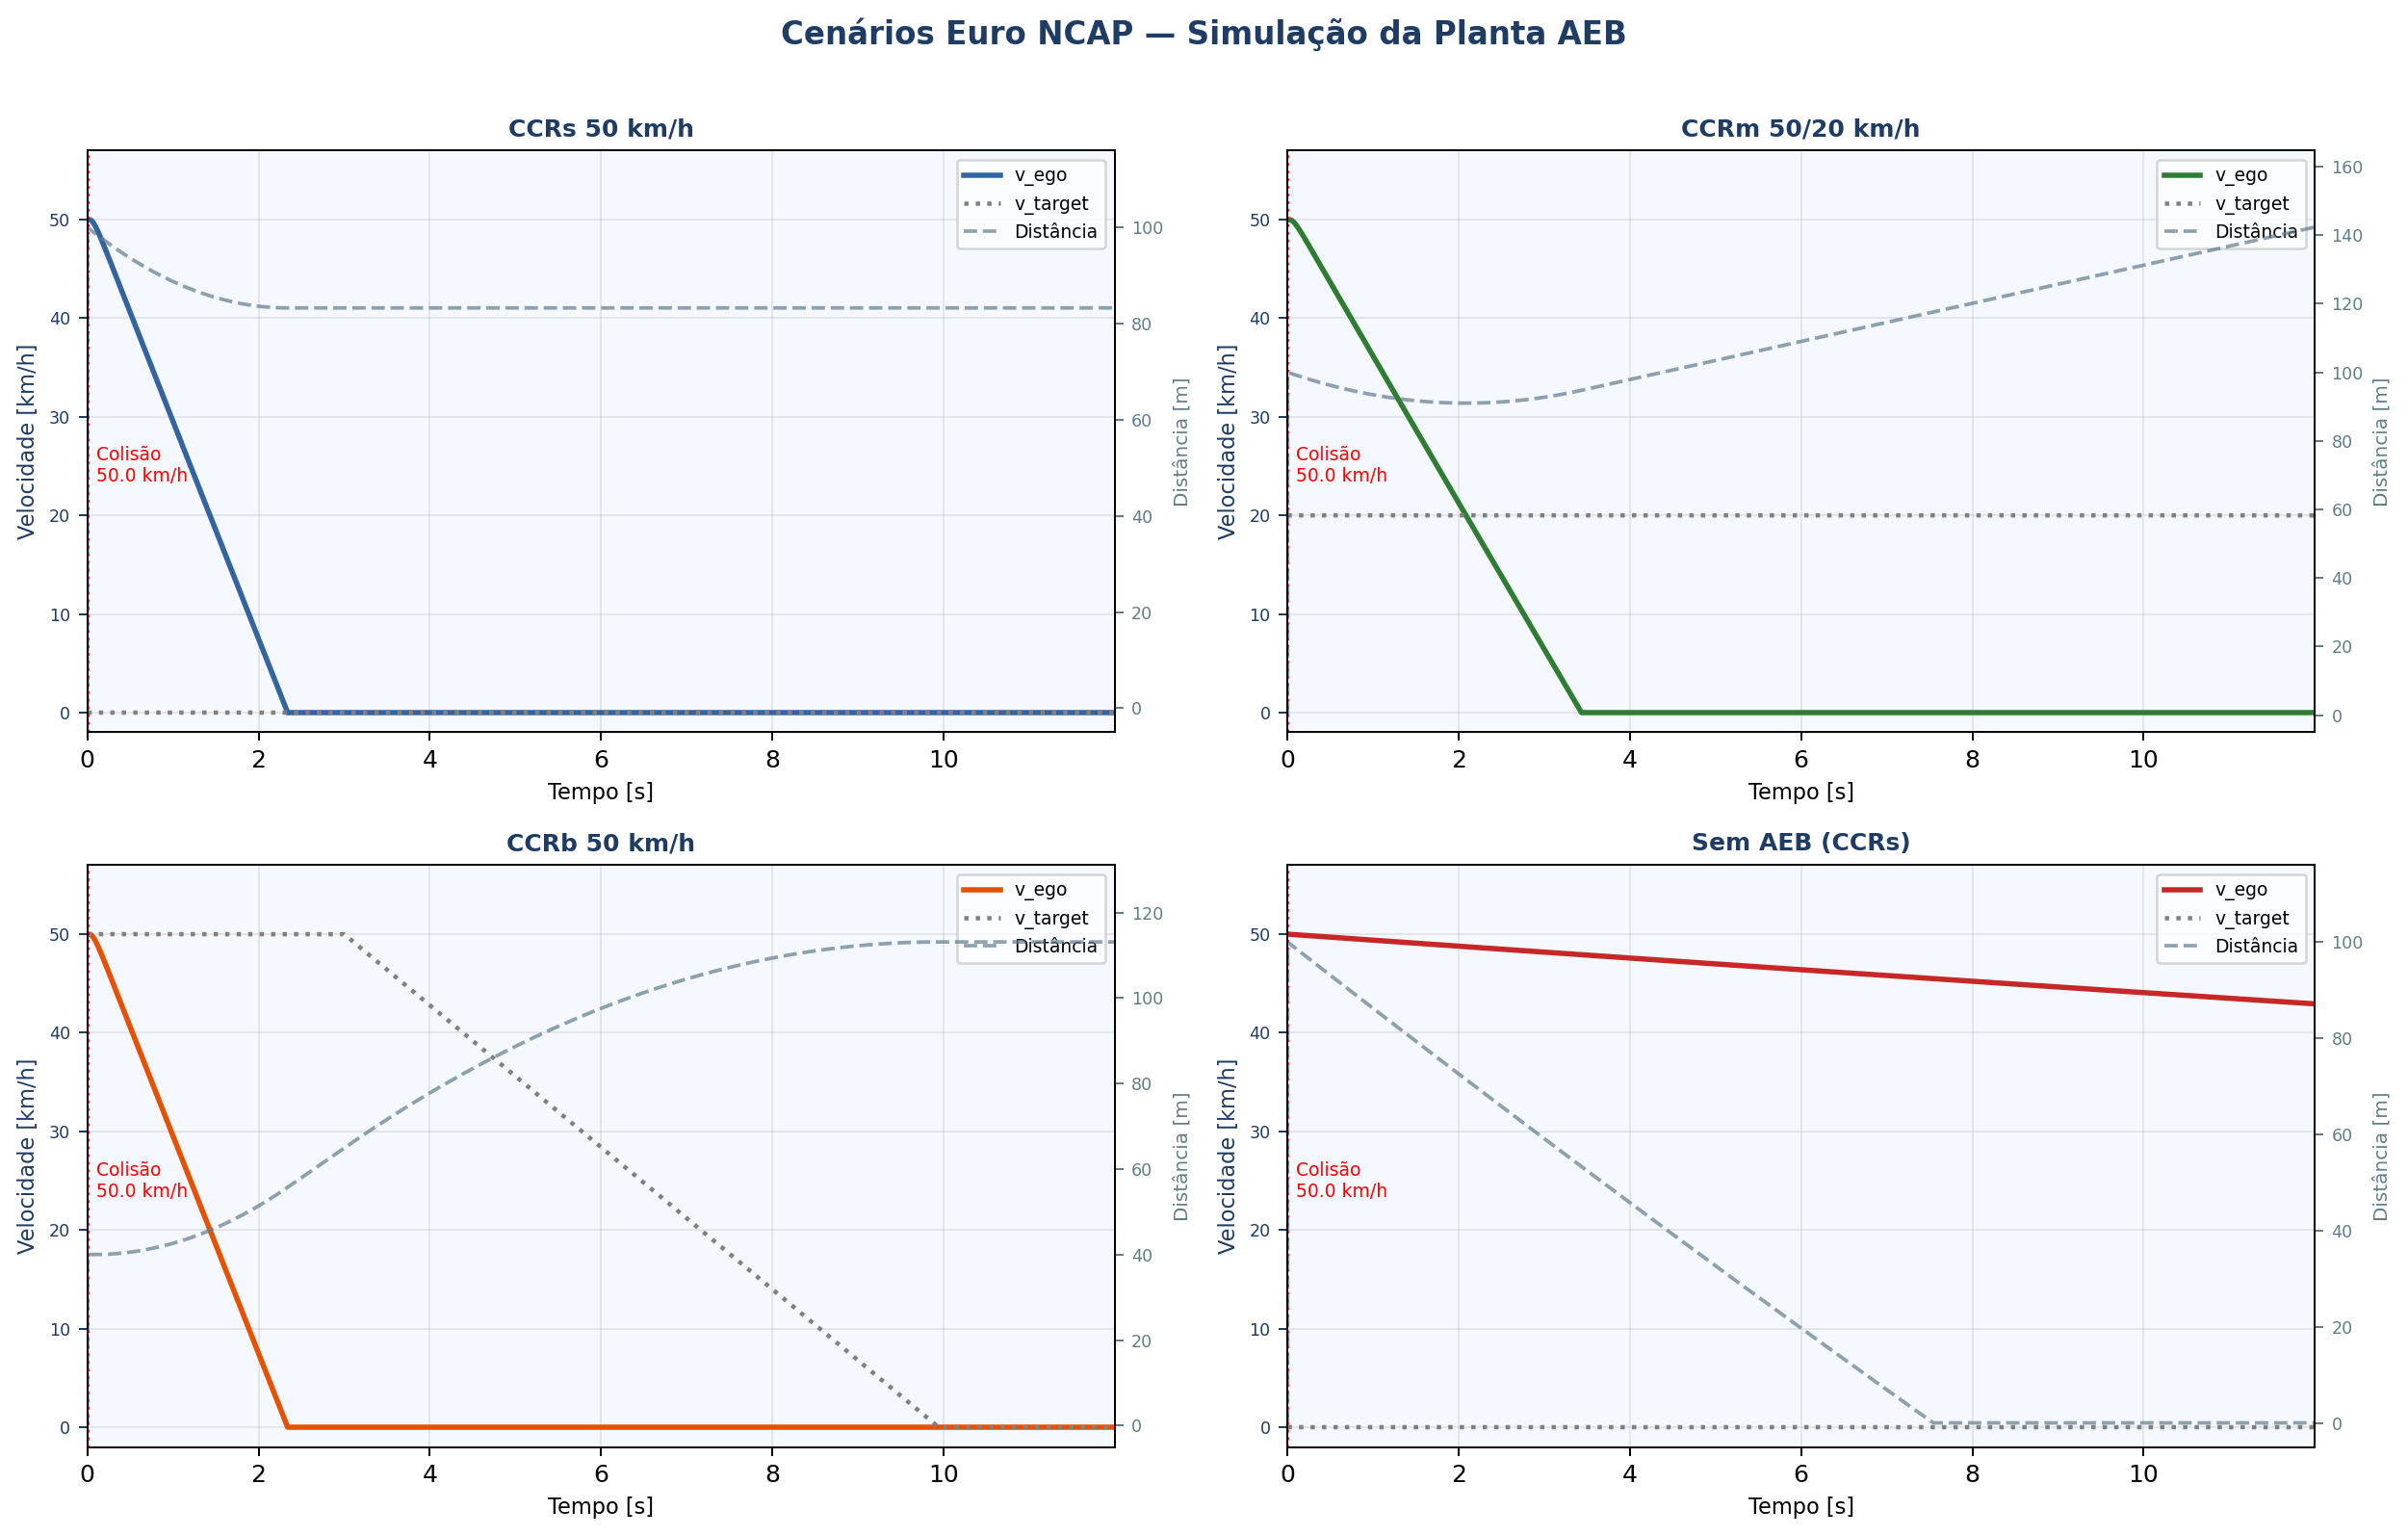
\includegraphics[width=\linewidth]{figs/fig_cenarios.png}
  \caption{Simulação numérica dos quatro cenários principais: velocidade e distância ao longo do tempo.}
  \label{fig:cenarios}
\end{figure}

\begin{table}[H]
  \centering
  \caption{Parâmetros dos cenários Euro NCAP implementados.}
  \begin{tabular}{lcccccc}
    \toprule
    \rowcolor{azulescuro!90}
    \color{white}\textbf{Cenário} &
    \color{white}\textbf{$v_\text{ego}$} &
    \color{white}\textbf{$v_\text{alvo}$} &
    \color{white}\textbf{Gap} &
    \color{white}\textbf{$a_\text{alvo}$} &
    \color{white}\textbf{$t_\text{brake}$} &
    \color{white}\textbf{TTC inicial} \\
    \midrule
    CCRs 20 & 20\,km/h & 0       & 40\,m  & 0              & --   & 7,2\,s \\
    \rowcolor{azulclaro!50}
    CCRs 30 & 30\,km/h & 0       & 60\,m  & 0              & --   & 7,2\,s \\
    CCRs 40 & 40\,km/h & 0       & 80\,m  & 0              & --   & 7,2\,s \\
    \rowcolor{azulclaro!50}
    CCRs 50 & 50\,km/h & 0       & 100\,m & 0              & --   & 7,2\,s \\
    CCRm    & 50\,km/h & 20\,km/h& 100\,m & 0              & --   & 12\,s  \\
    \rowcolor{azulclaro!50}
    CCRb    & 50\,km/h & 50\,km/h& 40\,m  & $-2$\,m/s²    & 3\,s & $\infty$\\
    CCRb hard& 50\,km/h& 50\,km/h& 40\,m  & $-6$\,m/s²    & 3\,s & $\infty$\\
    \rowcolor{azulclaro!50}
    no\_aeb & 50\,km/h & 0       & 100\,m & 0              & --   & 7,2\,s \\
    \bottomrule
  \end{tabular}
\end{table}

\begin{itemize}
  \item \textbf{CCRs} (\emph{Stationary}): alvo estacionário. Representa $\approx 80$\%
        dos acidentes traseiros urbanos. A faixa 20--50\,km/h cobre o espectro da
        UNECE~R152 (10--60\,km/h).

  \item \textbf{CCRm} (\emph{Moving}): alvo em movimento mais lento. A diferença de
        30\,km/h ($= 8{,}33$\,m/s) é representativa de congestionamentos urbanos.

  \item \textbf{CCRb} (\emph{Braking}): cenário mais complexo --- ambos os veículos
        trafegam à mesma velocidade e o alvo freia abruptamente. Desaceleração de
        $-2$\,m/s² é o baseline Euro NCAP; $-6$\,m/s² é o teste extremo.

  \item \textbf{no\_aeb}: cenário de referência sem frenagem. O ego mantém velocidade
        constante e colide com o alvo. Útil como \emph{baseline} de comparação.
\end{itemize}

% ================================================================
\section{Parâmetros de Simulação}
\label{sec:sim}

\begin{table}[H]
  \centering
  \caption{Configuração do solver e tempo de simulação.}
  \begin{tabularx}{\linewidth}{lclX}
    \toprule
    \rowcolor{azulescuro!90}
    \color{white}\textbf{Parâmetro} & \color{white}\textbf{Valor} &
    \color{white}\textbf{Unidade} & \color{white}\textbf{Justificativa} \\
    \midrule
    \param{SIM\_STOP\_TIME} & 15 & s &
      Suficiente para CCRs 50\,km/h: $100/13{,}89 \approx 7{,}2$\,s + margem POST\_BRAKE. \\
    \rowcolor{azulclaro!50}
    \param{SIM\_DT}         & 1  & ms &
      Resolução 50$\times$ maior que o ciclo de controle (10\,ms). $\tau/dt = 50$ garante boa discretização do atuador. \\
    Solver                  & ode4 & -- &
      Runge-Kutta 4\textsuperscript{a} ordem, passo fixo. Determinístico --- essencial para SIL reprodutível. \\
    \bottomrule
  \end{tabularx}
\end{table}

\begin{notabox}[Por que passo fixo (ode4)?]
  Simulação SIL deve replicar o comportamento do código embarcado, que opera em
  ciclos determinísticos de 10\,ms. Um solver de passo variável (ex.: ode45) poderia
  ``pular'' eventos curtos ou introduzir assimetrias temporais não presentes no
  sistema real.
\end{notabox}

% ================================================================
\section{Equações do Modelo}
\label{sec:equacoes}

\begin{figure}[H]
  \centering
  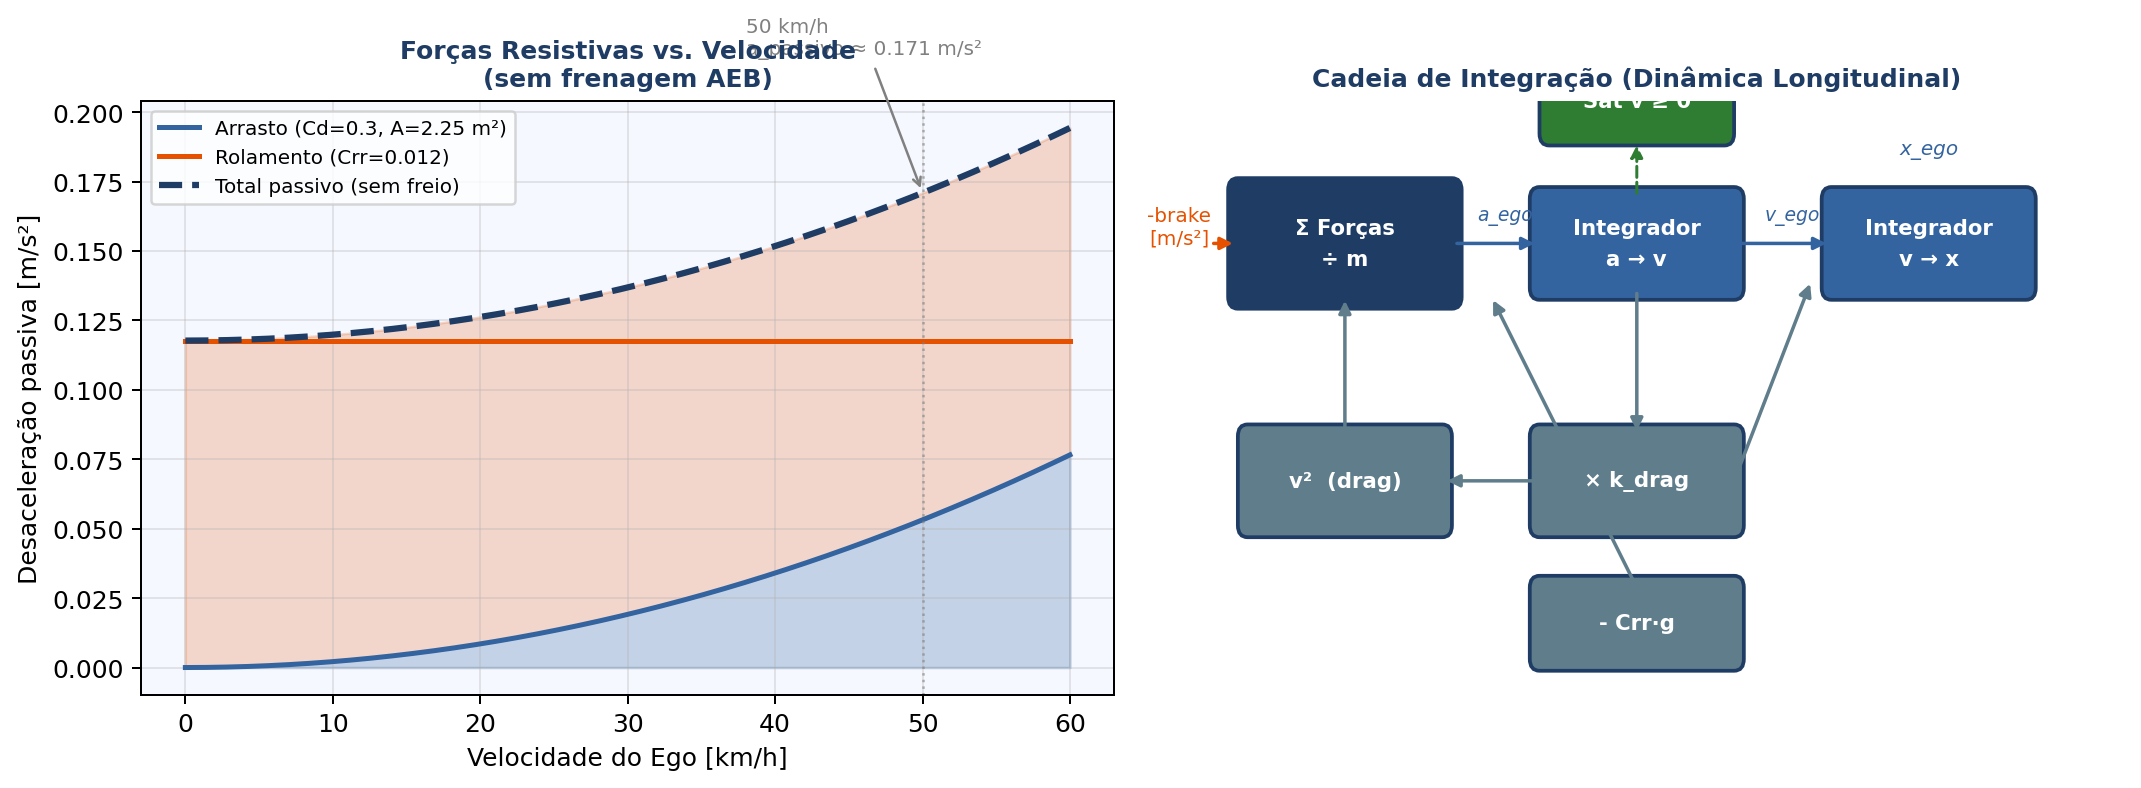
\includegraphics[width=\linewidth]{figs/fig_dinamica.png}
  \caption{Forças resistivas vs.\ velocidade (esq.) e cadeia de integração (dir.).}
  \label{fig:dinamica}
\end{figure}

\subsection{Dinâmica longitudinal do ego}

A equação de movimento longitudinal, somando todas as forças resistivas:

\begin{equation}
  m \cdot a_\text{ego} = -F_\text{brake} - F_\text{drag} - F_\text{roll} - F_\text{grade}
  \label{eq:newton}
\end{equation}

\begin{table}[H]
  \centering
  \begin{tabularx}{\linewidth}{llX}
    \toprule
    \rowcolor{azulescuro!90}
    \color{white}\textbf{Termo} & \color{white}\textbf{Equação} & \color{white}\textbf{Descrição} \\
    \midrule
    $F_\text{brake}$ & $a_\text{brake} \cdot m$ & Força de frenagem (AEB) \\
    \rowcolor{azulclaro!50}
    $F_\text{drag}$  & $\tfrac{1}{2}\,C_d \cdot A \cdot \rho \cdot v_\text{ego}^2$ & Resistência aerodinâmica \\
    $F_\text{roll}$  & $C_{rr} \cdot m \cdot g$ & Resistência ao rolamento \\
    \rowcolor{azulclaro!50}
    $F_\text{grade}$ & $m \cdot g \cdot \sin\!\left(\arctan\!\tfrac{\text{grade}}{100}\right)$ & Componente gravitacional \\
    \bottomrule
  \end{tabularx}
\end{table}

Dividindo a Eq.~\eqref{eq:newton} por $m$:

\begin{equation}
  a_\text{ego} = -a_\text{brake}
               - \underbrace{\frac{C_d\, A\, \rho}{2m}}_{k_\text{drag}} v_\text{ego}^2
               - C_{rr}\, g
               - g\,\sin\!\left(\arctan\frac{\text{grade}}{100}\right)
\end{equation}

A 50\,km/h com $m = 1500$\,kg: $k_\text{drag} = \frac{0{,}3 \times 2{,}25 \times 1{,}225}{2 \times 1500} \approx 2{,}76 \times 10^{-4}$\,m$^{-1}$.

\subsection{Integração numérica}

\begin{align}
  v_\text{ego}(t) &= \int a_\text{ego}\, dt, \quad v_\text{ego} \geq 0 \\
  x_\text{ego}(t) &= \int v_\text{ego}\, dt, \quad x_\text{ego}(0) = 0
\end{align}

A condição $v_\text{ego} \geq 0$ é imposta por um bloco \emph{Saturation} --- o veículo não anda para trás.

\subsection{Cinemática relativa}

\begin{align}
  d(t)       &= \max\!\left(0,\; x_\text{alvo}(t) - x_\text{ego}(t)\right) \\
  v_\text{rel}(t) &= v_\text{ego}(t) - v_\text{alvo}(t)
\end{align}

O controlador AEB calcula o TTC a partir desses sinais via CAN:
\[
  \text{TTC}(t) = \frac{d(t)}{v_\text{rel}(t)}, \quad v_\text{rel} > 0
\]

\subsection{Perfil de velocidade do alvo}

\begin{equation}
  v_\text{alvo}(t) =
  \begin{cases}
    v_{\text{alvo},0} & \text{se } t < t_\text{brake} \\
    \max\!\left(0,\; v_{\text{alvo},0} + a_\text{alvo} \cdot (t - t_\text{brake})\right) & \text{se } t \geq t_\text{brake}
  \end{cases}
\end{equation}

% ================================================================
\section{TTC e Evolução da FSM}
\label{sec:ttc}

\begin{figure}[H]
  \centering
  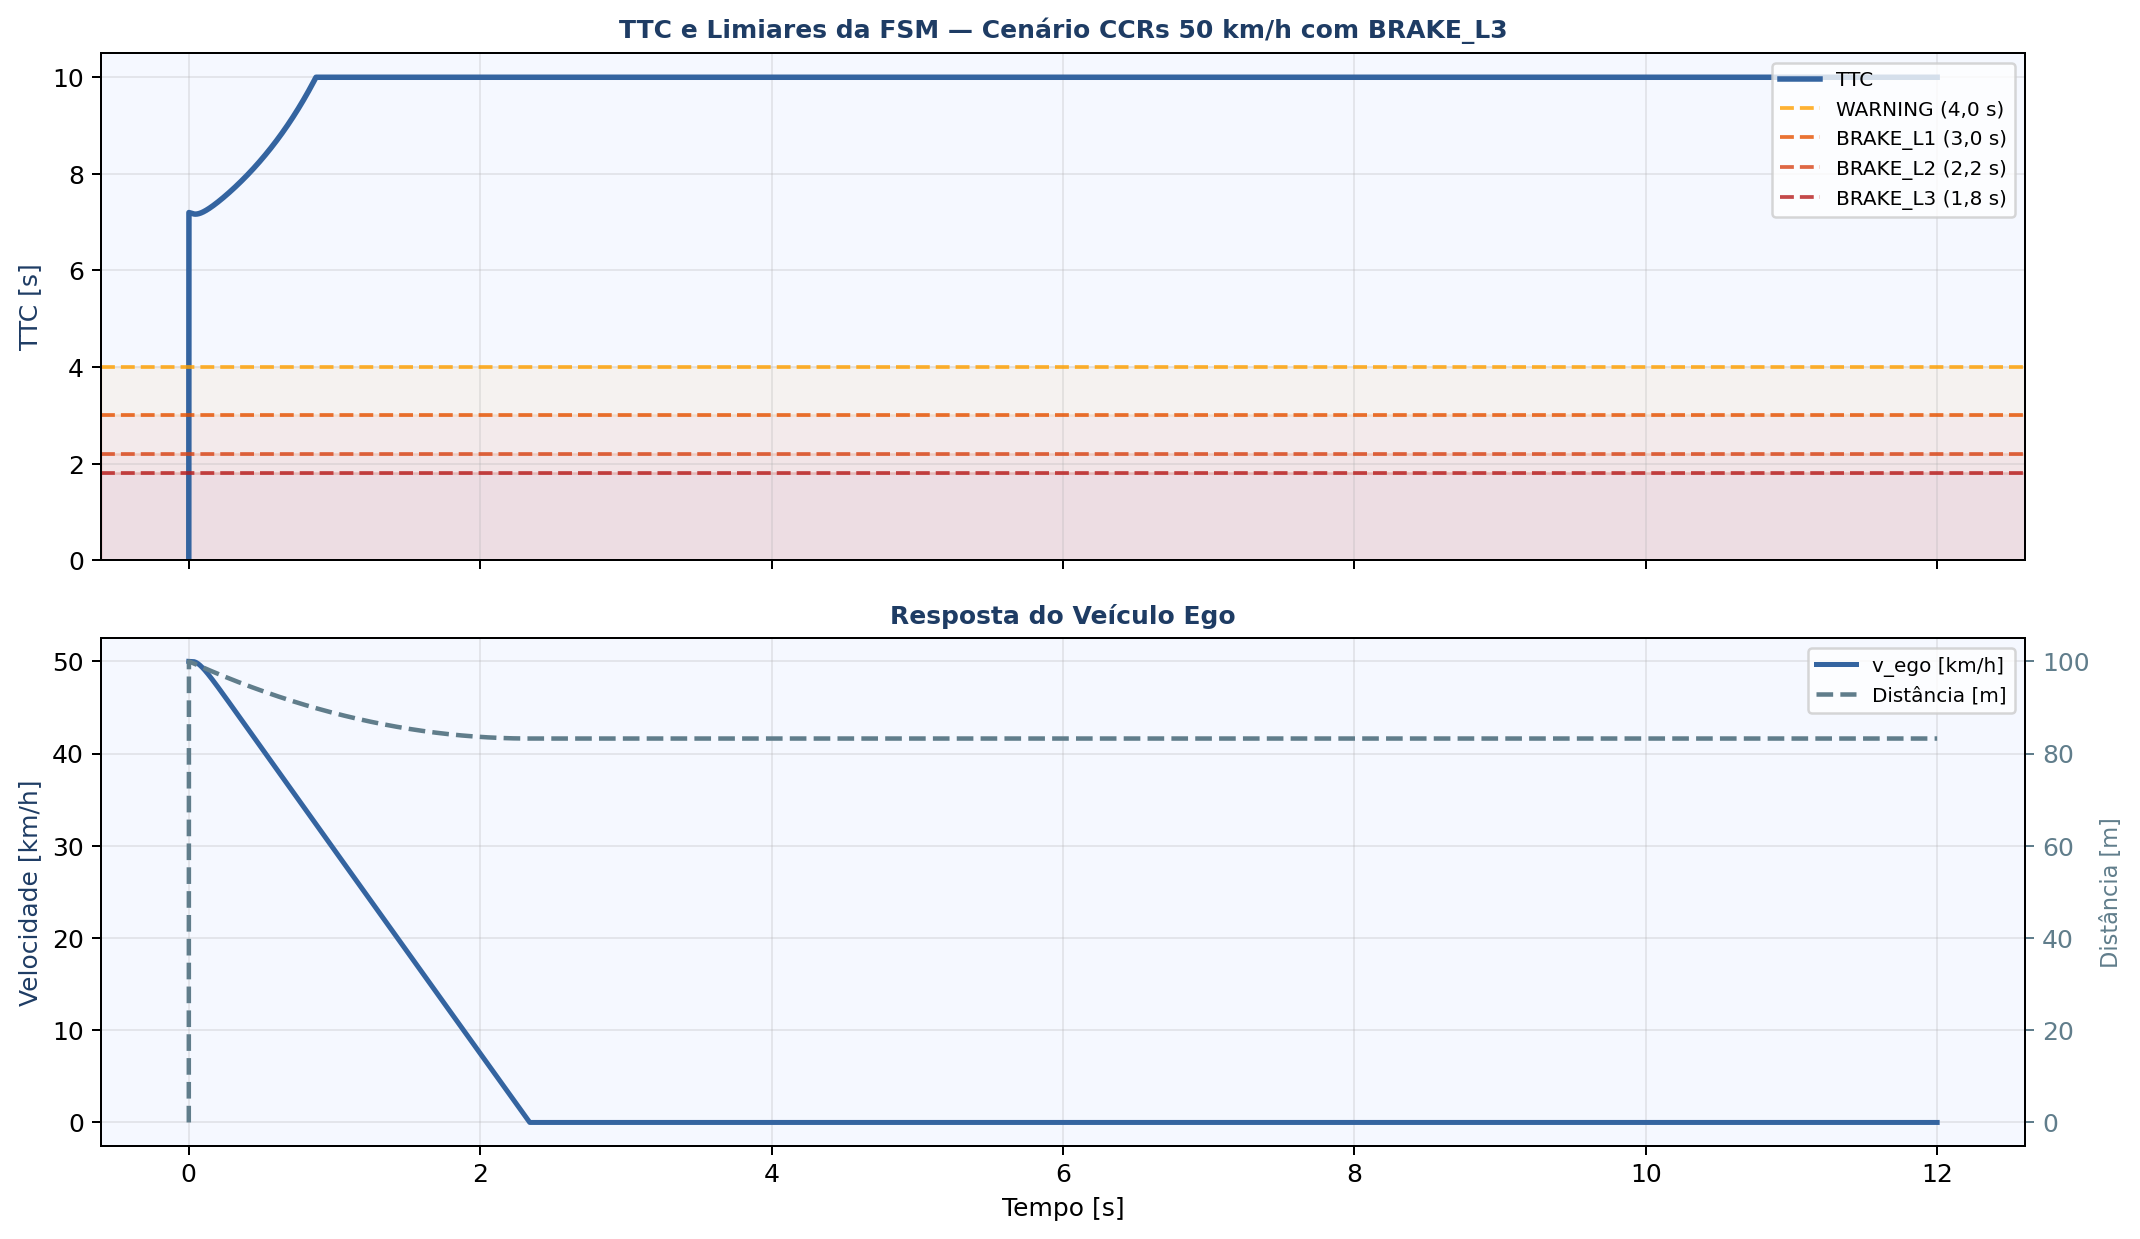
\includegraphics[width=\linewidth]{figs/fig_ttc.png}
  \caption{Evolução do TTC e limiares da FSM no cenário CCRs 50\,km/h com frenagem BRAKE\_L3.}
  \label{fig:ttc}
\end{figure}

A Figura~\ref{fig:ttc} mostra como o TTC diminui ao longo do tempo e cruza os limiares
da Máquina de Estados (FSM), provocando as transições:
\textbf{STANDBY $\to$ WARNING $\to$ BRAKE\_L1 $\to$ BRAKE\_L2 $\to$ BRAKE\_L3}.

A planta fornece os sinais de distância e velocidade relativa que permitem ao controlador
calcular este TTC. Os limiares da FSM estão definidos em \texttt{aeb\_config.h}:

\begin{table}[H]
  \centering
  \begin{tabular}{lcc}
    \toprule
    \rowcolor{azulescuro!90}
    \color{white}\textbf{Estado} & \color{white}\textbf{TTC limiar} & \color{white}\textbf{Desaceleração} \\
    \midrule
    WARNING    & $\leq 4{,}0$\,s & 0\,m/s² \\
    \rowcolor{azulclaro!50}
    BRAKE\_L1  & $\leq 3{,}0$\,s & 2\,m/s² \\
    BRAKE\_L2  & $\leq 2{,}2$\,s & 4\,m/s² \\
    \rowcolor{azulclaro!50}
    BRAKE\_L3  & $\leq 1{,}8$\,s & 6\,m/s² \\
    \bottomrule
  \end{tabular}
\end{table}

% ================================================================
\section{Simplificações e Limitações}
\label{sec:simplif}

\begin{table}[H]
  \centering
  \caption{Simplificações adotadas e seus impactos.}
  \begin{tabularx}{\linewidth}{lXX}
    \toprule
    \rowcolor{azulescuro!90}
    \color{white}\textbf{Simplificação} &
    \color{white}\textbf{Justificativa} &
    \color{white}\textbf{Impacto} \\
    \midrule
    Modelo 1D longitudinal &
      AEB controla apenas o eixo longitudinal. &
      Nenhum para cenários CCR em linha reta. \\
    \rowcolor{azulclaro!50}
    Atrito constante ($\mu = 0{,}85$) &
      Testes Euro NCAP em asfalto seco. &
      Ajustar \param{BRAKE\_MAX\_DECEL} para chuva/neve. \\
    Mapeamento linear pressão-decel. &
      Simplifica curva não-linear do sistema de freios. &
      Aceitável para SIL; produção usaria \emph{lookup table}. \\
    \rowcolor{azulclaro!50}
    Sem transferência de carga &
      Simplifica dinâmica de pitch/roll. &
      Impacto $< 5$\% na desaceleração. \\
    Sem modelo de pneu &
      Desnecessário para SIL acadêmico. &
      Pneu implícito via \param{BRAKE\_MAX\_DECEL}. \\
    \rowcolor{azulclaro!50}
    $C_{rr}$ constante &
      Variação $< 10$\% na faixa 5--60\,km/h. &
      Aceitável para eventos de curta duração. \\
    \bottomrule
  \end{tabularx}
\end{table}

Estas simplificações são adequadas para o objetivo do modelo: \textbf{validação SIL
do algoritmo do controlador AEB embarcado em C}. Um modelo de maior fidelidade
(HIL ou veículo real) requereria Magic Formula, transferência de carga, modelo
de suspensão e mapa não-linear do sistema de freios.

% ================================================================
\section{Referências}
\label{sec:refs}

\begin{enumerate}
  \item Euro NCAP. \textit{AEB Car-to-Car Test Protocol}, Version 4.3. Brussels, 2023.

  \item UNECE. \textit{Regulation No.~152 --- Uniform provisions concerning the approval
        of motor vehicles with respect to AEBS}. Geneva, 2021.

  \item SAE International. \textit{J2452: Stepwise Coastdown Methodology for Measuring
        Tire Rolling Resistance}. 2017.

  \item Bosch Mobility. \textit{iBooster --- Electromechanical Brake Booster}.
        Product Description, 2022.

  \item MathWorks. \textit{Automated Emergency Braking Test Bench}.
        MATLAB/Simulink Automotive Reference Application, R2025b.

  \item Reif, K. (Ed.). \textit{Brakes, Brake Control and Driver Assistance Systems}.
        Springer Vieweg, 2014.

  \item Rajamani, R. \textit{Vehicle Dynamics and Control}. 2ª~ed. Springer, 2012.

  \item MDPI Applied Sciences. ``Optimizing AEB Thresholds for NCAP''. Vol.~13, 2023.

  \item \texttt{c\_embedded/include/aeb\_config.h} --- Projeto AEB, parâmetros do controlador.
\end{enumerate}

\end{document}
